\subsubsection{UC13 - Log funzioni eseguite}
\begin{figure}[h]
	\centering
	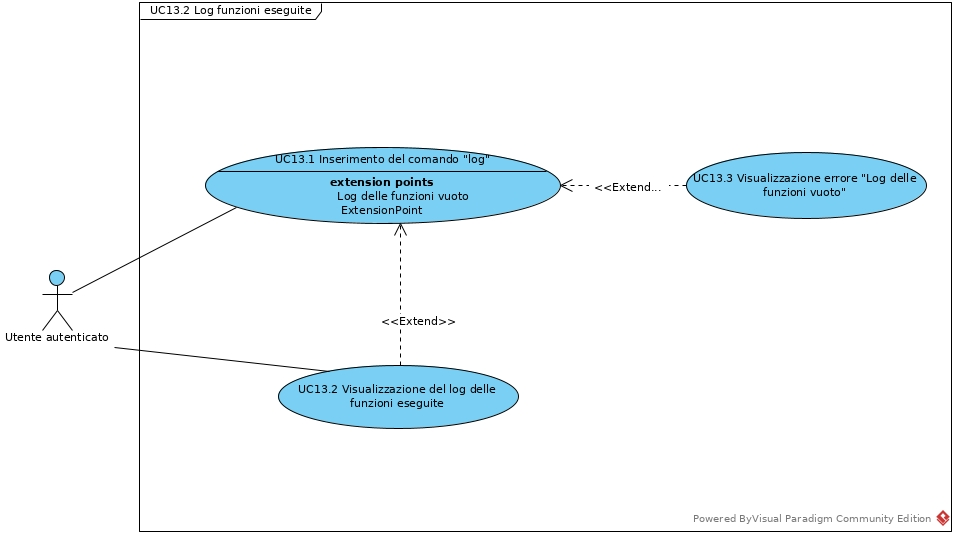
\includegraphics[width=\linewidth]{res/img/UC13.jpg}
	\caption{Diagramma UC13 - Log funzioni eseguite}
\end{figure}
\begin{itemize}
	\item \textbf{Attori primari:} Utente autenticato;
	\item \textbf{Descrizione:} l'utente prova a visualizzare il log delle funzioni da lui eseguite mediante l'apposito comando "log";
	\item \textbf{Pre-condizioni:} l'utente ha utilizzato il comando per la visualizzazione del log;
	\item \textbf{Post-condizioni:} il sistema visualizzerà sulla \textit{CLI\glo} il log delle funzioni eseguite dall'utente oppure visualizzerà sulla schermata "Log funzioni vuote";
	\begin{itemize}
		\item \textbf{UC13.2}: l'inserimento del comando "log" provoca la visualizzazione di risulati tramite \textit{CLI\glos}.
	\end{itemize}
	\item \textbf{Estensioni:}
	\begin{itemize}
		\item \textbf{UC13.3}: se l'utente non ha eseguito ancora alcuna funzione tra quelle presenti nel sistema \textit{Etherless\glos}, verrà restituito un messaggio di errore.
	\end{itemize}
\end{itemize}
